\section{Analysis of the synthetic axion data}
After TASEH finished collecting the CD102 data on November 15, 2021, 
the synthetic axion signals were injected into the cavity and read out via the 
same transmission line and amplification chain. The procedure 
to generate axion-like signals is summarized in 
Ref.~\cite{TASEHInstrumentation}. 
Due to the uncertainties on the losses of readout electronics and transmission
 lines, the synthetic axion signals were not used to perform an absolute 
calibration of search sensitivity. Instead, 
a test with synthetic axion signals could be used to verify the procedures of 
data acquisition and physics analysis. The 
signal-to-noise ratio (SNR) of the frequency bin with maximum power, at 
4.708972~GHz, was set to $\approx 3.35\sigma$, corresponding to 
a power of $\approx 6.03 \times 10^{-13}$~W in a 1-kHz frequency bin.  

Figures~\ref{fig:faxionstep}--\ref{fig:faxionmerge} present respectively the 
power spectra in 24 frequency scans, the spectrum after combining the 24 
spectra vertically, and the spectrum after merging five neighboring bins with 
a signal line shape following Eq.~(\ref{eq:simplesignal}). Before combining 
the 24 spectra vertically, the SNR of the maximum-power bin from the spectrum 
with a cavity resonant frequency of 4.708918~GHz was measured to be 
3.577$\sigma$; the SNR was slightly higher than 3.35$\sigma$ due to a 
5\% difference in the noise fluctuation between the measurements from 
the HEMT calibration and the measurements taken 
right before injecting axion-like signals. After the vertical combination 
of power spectra and the merging of five frequency bins, the SNR increased to 
4.74$\sigma$ and 6.12$\sigma$, respectively. 
The analysis results of the synthetic axion signals proved that an power 
excess of more than 5$\sigma$ can be found at the expected frequencies via 
the standard analysis procedure.  

\begin{figure}[htbp]                                                                                                  
    \centering                                                                                                                       
%    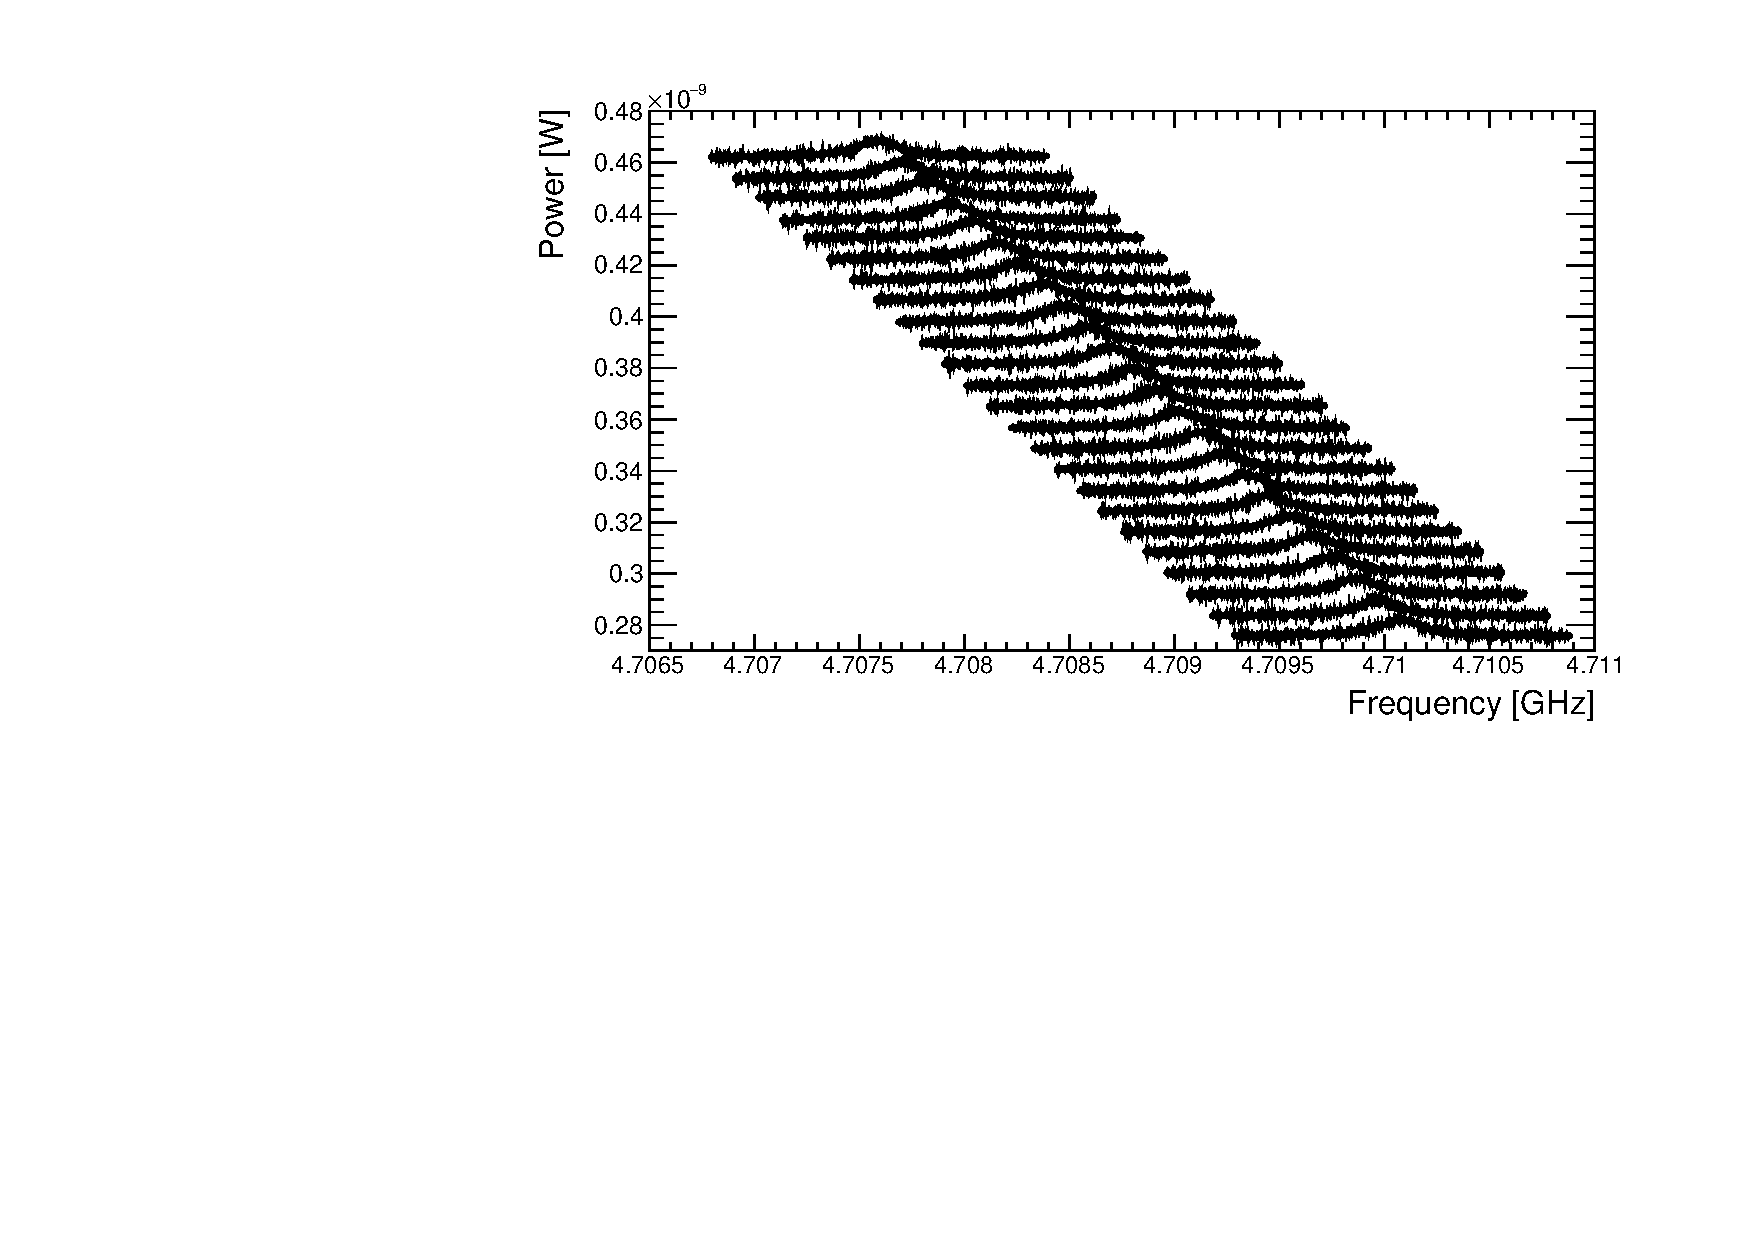
\includegraphics[width=0.48\textwidth]{figures/RawSpectra_Faxion_YAxis_Shifted.pdf}
    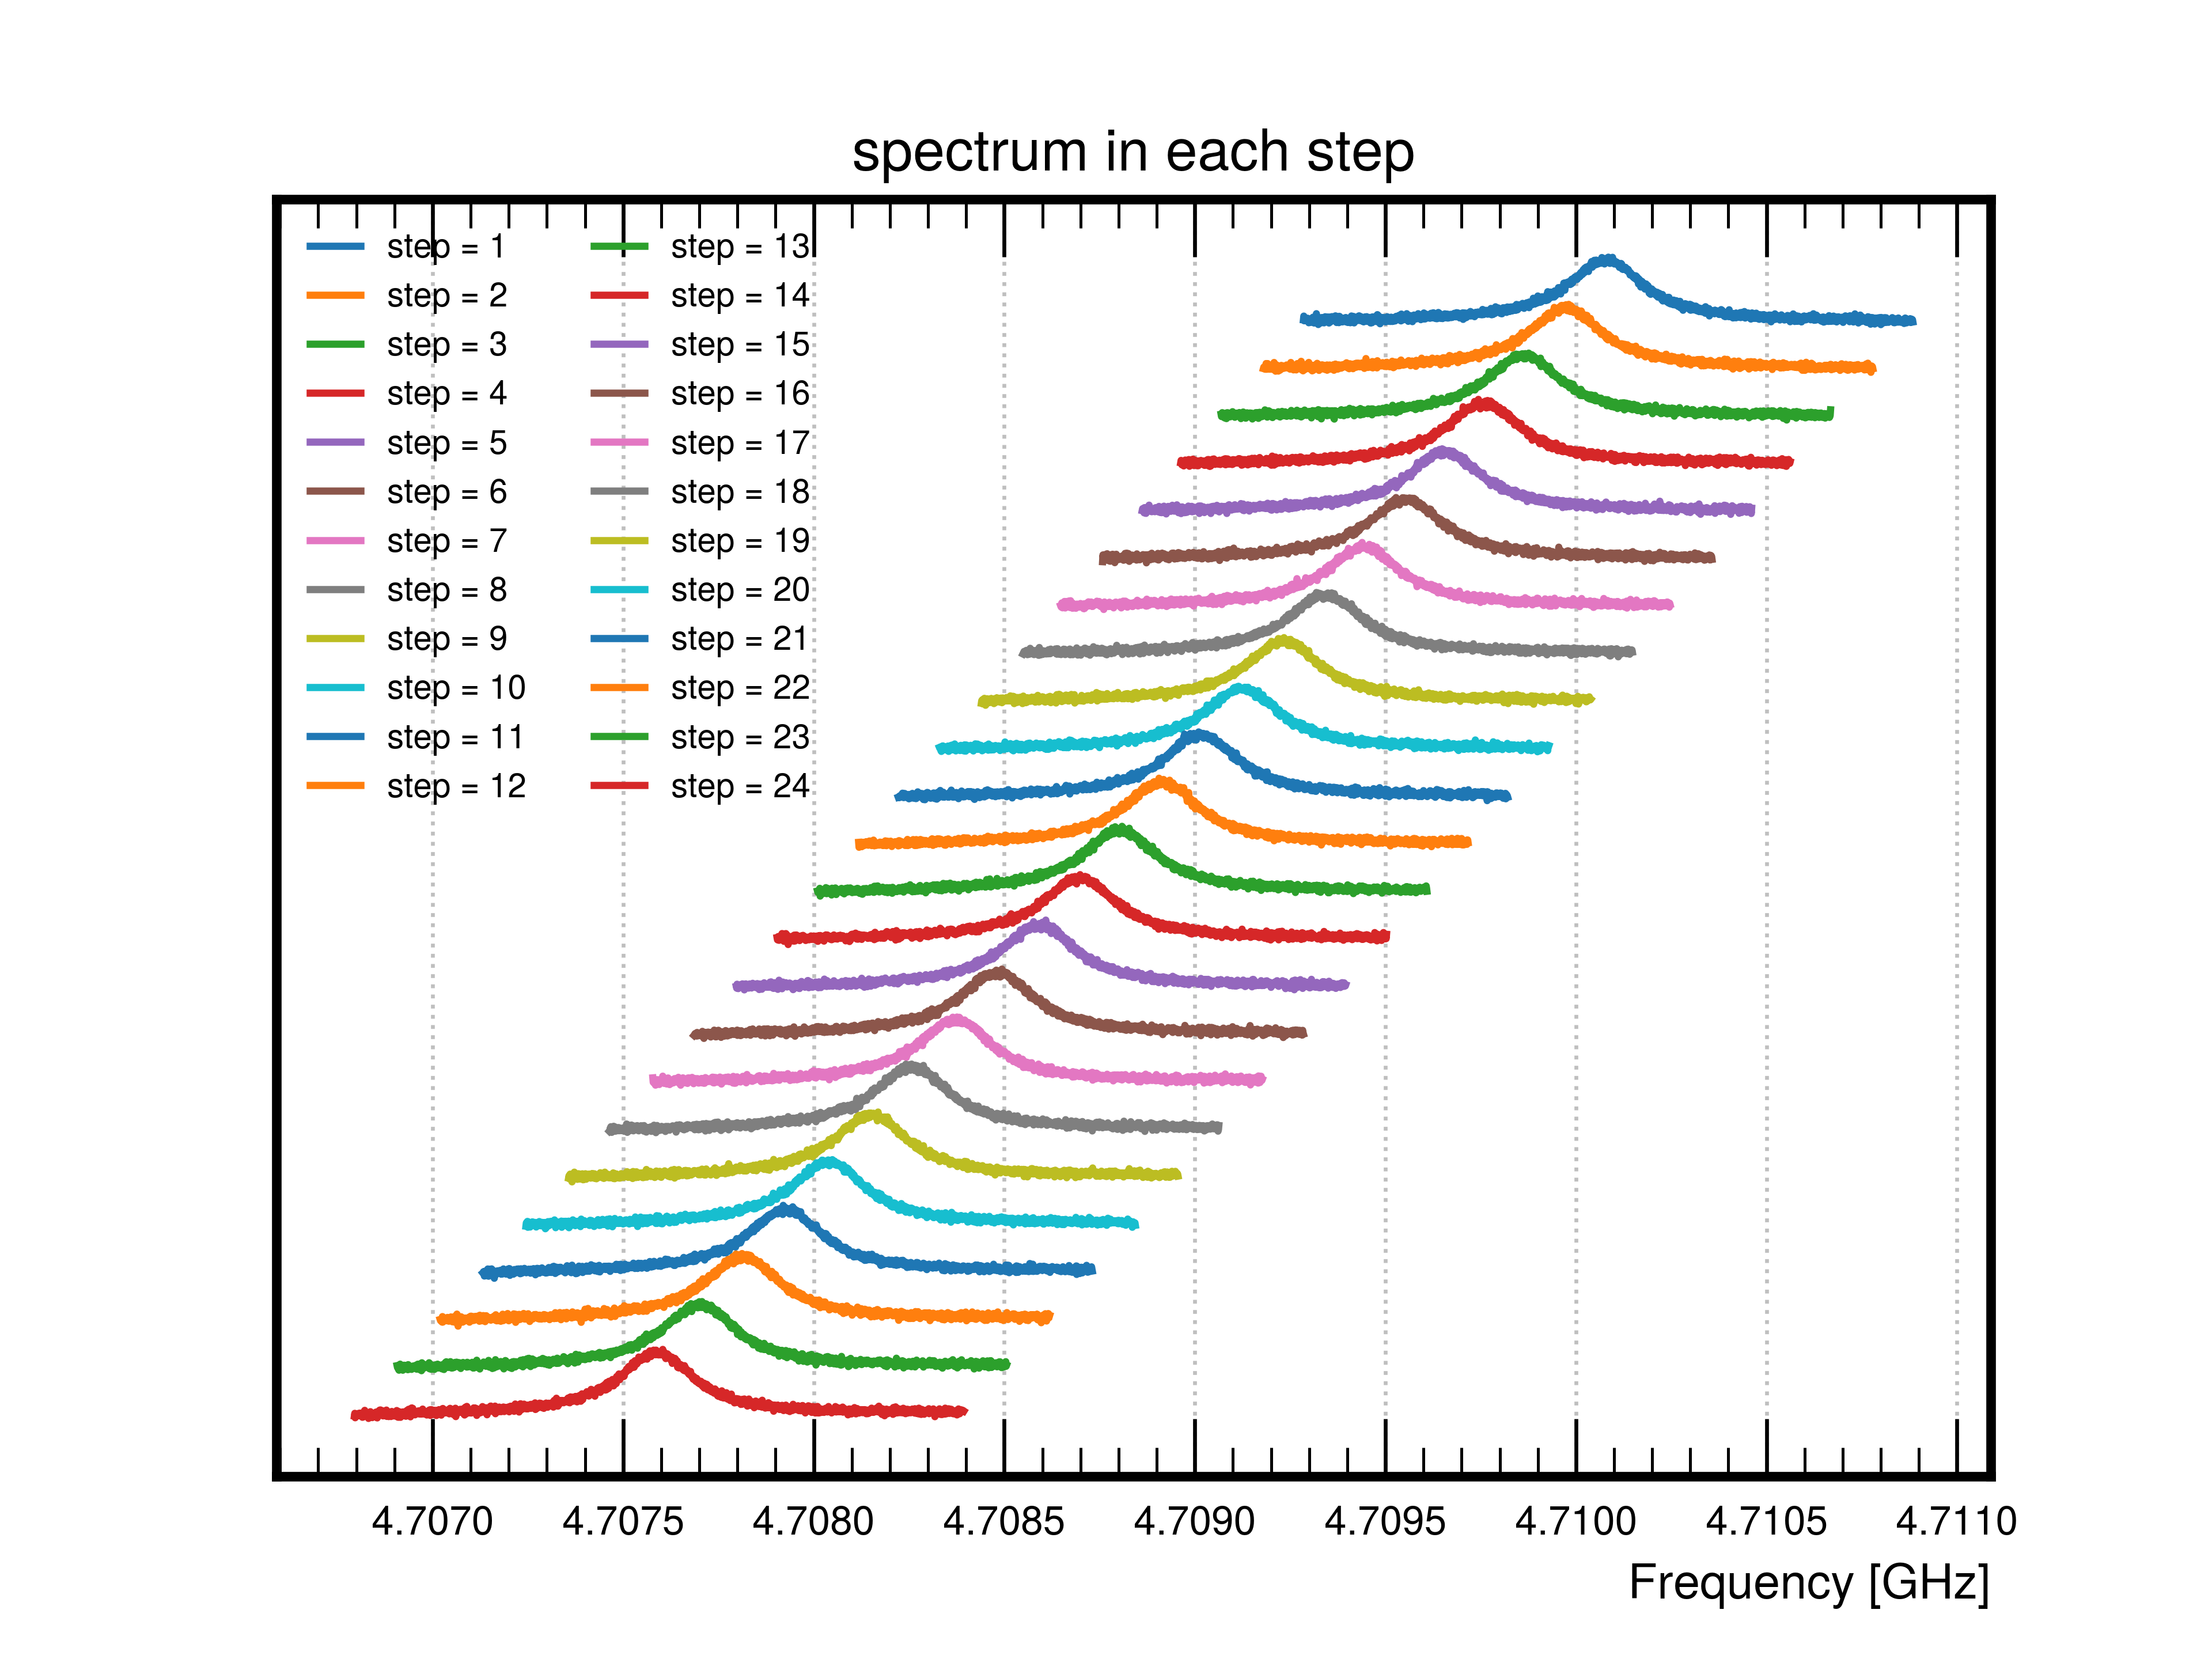
\includegraphics[width=8.6cm]{figures/faxion_rawpower_24steps.png}
 \caption{The power spectra, before removing the gain of the receiver and applying the 
 SG filter, from the 24 frequency steps of the synthetic axion 
data. In order to show the spectra clearly, the spectra are shifted 
with respect to each other with an arbitrary offset in the vertical scale.}                
\label{fig:faxionstep}                                                                                                            
\end{figure}                       

\begin{figure}[htbp]                                                                                                  
    \centering                                                                                                                       
    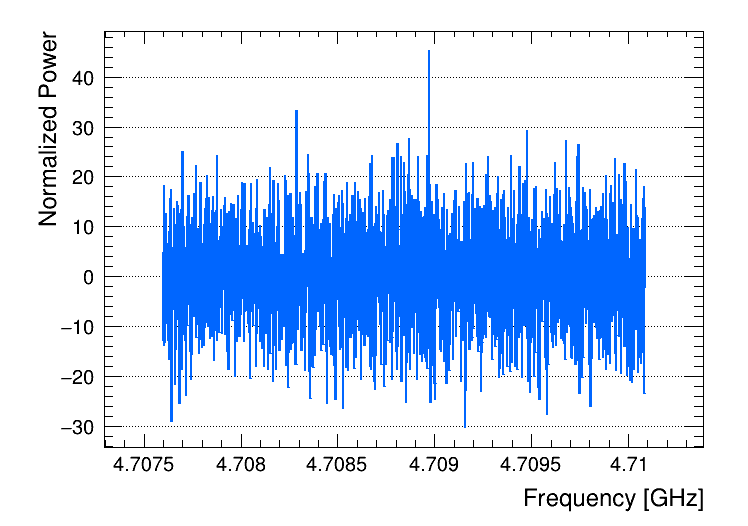
\includegraphics[width=0.48\textwidth]{figures/Power_CombSpectrum_FaxionRun_AllSteps_Rescan_SG4_W201.png}
    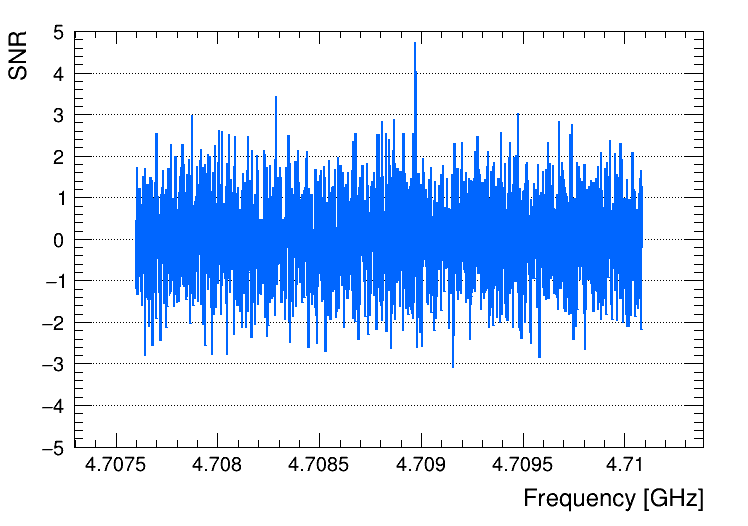
\includegraphics[width=0.48\textwidth]{figures/SNR_CombSpectrum_FaxionRun_AllSteps_Rescan_SG4_W201.png}
    \caption{The power (left) and signal-to-noise ratio (right) after combining the spectra with overlapping 
frequencies vertically. The procedure and the weights for combination 
are summarized in Section~\ref{sec:ana}.}                
\label{fig:faxioncombine}                                                                                                            
\end{figure}                       


\begin{figure}[htbp]                                                                                                  
    \centering                                                                                                                       
    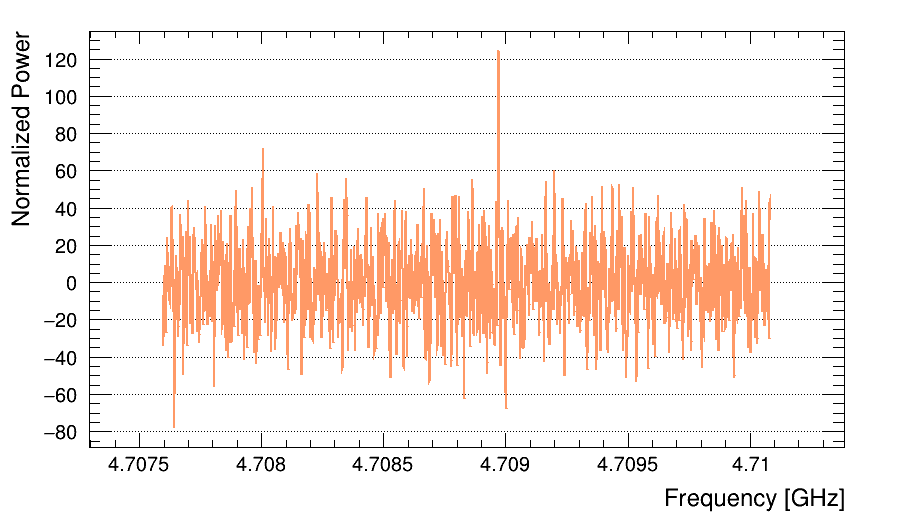
\includegraphics[width=0.48\textwidth]{figures/Power_GrandSpectrum_FaxionRun_AllSteps_Rescan_Merged_5bin_SG4_W201_LqWeight.png}
    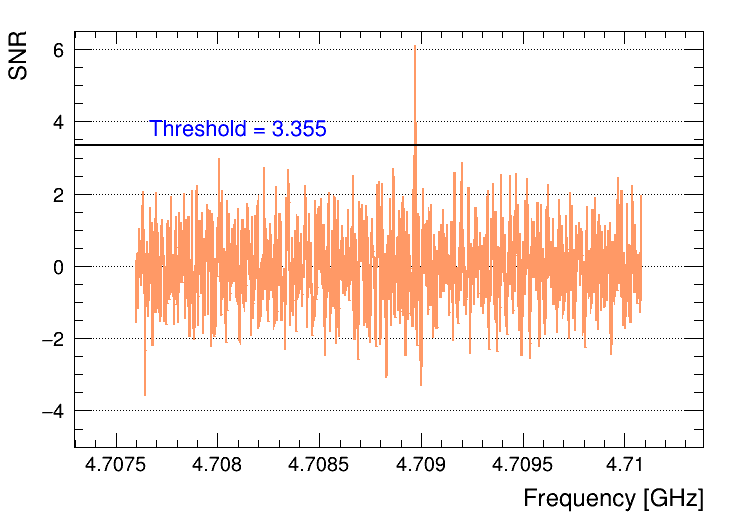
\includegraphics[width=0.48\textwidth]{figures/SNR_GrandSpectrum_FaxionRun_AllSteps_Rescan_Merged_5bin_SG4_W201_LqWeight.png}
    \caption{The power (left) and signal-to-noise ratio (right) after merging the power measured in five 
neighboring frequency bins. The procedure and the weights for merging 
are summarized in Section~\ref{sec:ana}.}                
\label{fig:faxionmerge}    
\end{figure}                       

   
